\documentclass[10pt,a5paper]{article}
\usepackage[utf8]{inputenc}
\usepackage[english]{babel}
\usepackage{amsmath}
\usepackage{amsfonts}
\usepackage{amssymb}
\usepackage{graphicx}
\usepackage{lmodern}
\usepackage[left=0.25cm,right=0.25cm,top=0.25cm,bottom=0.25cm,paperwidth=11.5cm,paperheight=11.75cm]{geometry}
\usepackage{tikz}
\usetikzlibrary{decorations.pathreplacing,angles,quotes}
\usetikzlibrary{shapes}
\pgfdeclarelayer{background}
\pgfdeclarelayer{foreground}
\pgfsetlayers{background,main,foreground}

\definecolor{darkred}{rgb}{0.7,0,0}

%%%% taken from
% https://tex.stackexchange.com/questions/267222/3d-arrows-with-tikz
\usepgflibrary{arrows.meta}
\makeatletter
\pgfkeys{
  /pgf/arrow keys/.cd,
  pitch/.code={%
    \pgfmathsetmacro\pgfarrowpitch{#1}
    \pgfmathsetmacro\pgfarrowsinpitch{abs(sin(\pgfarrowpitch))}
    \pgfmathsetmacro\pgfarrowcospitch{abs(cos(\pgfarrowpitch))}
  },
}

\pgfdeclarearrow{
  name = Cone,
  defaults = {       % inherit from Kite
    length     = +1.pt +3,
    width'     = +0pt +0.6,
    line width = +0pt 1 1,
    pitch      = +0, % lie on screen
  },
  cache = false,     % no need cache
  setup code = {},   % so no need setup
  drawing code = {   % but still need math
    % draw the base
    \pgfmathsetmacro\pgfarrowhalfwidth{.5\pgfarrowwidth}
    \pgfmathsetmacro\pgfarrowhalfwidthsin{\pgfarrowhalfwidth*\pgfarrowsinpitch}
    \pgfpathellipse{\pgfpointorigin}{\pgfqpoint{\pgfarrowhalfwidthsin pt}{0pt}}{\pgfqpoint{0pt}{\pgfarrowhalfwidth pt}}
    \pgfusepath{fill}
    % test if the cone part visible
    \pgfmathsetmacro\pgfarrowlengthcos{\pgfarrowlength*\pgfarrowcospitch}
    \pgfmathparse{\pgfarrowlengthcos>\pgfarrowhalfwidthsin}
    \ifnum\pgfmathresult=1
      % it is visible, so draw
      \pgfmathsetmacro\pgfarrowlengthtemp{\pgfarrowhalfwidthsin*\pgfarrowhalfwidthsin/\pgfarrowlengthcos}
      \pgfmathsetmacro\pgfarrowwidthtemp{\pgfarrowhalfwidth/\pgfarrowlengthcos*sqrt(\pgfarrowlengthcos*\pgfarrowlengthcos-\pgfarrowhalfwidthsin*\pgfarrowhalfwidthsin)}
      \pgfpathmoveto{\pgfqpoint{\pgfarrowlengthcos pt}{0pt}}
      \pgfpathlineto{\pgfqpoint{\pgfarrowlengthtemp pt}{ \pgfarrowwidthtemp pt}}
      \pgfpathlineto{\pgfqpoint{\pgfarrowlengthtemp pt}{-\pgfarrowwidthtemp pt}}
      \pgfpathclose
      \pgfusepath{fill}
    \fi
    \pgfpathmoveto{\pgfpointorigin}
  }
}



\begin{document}
\centering
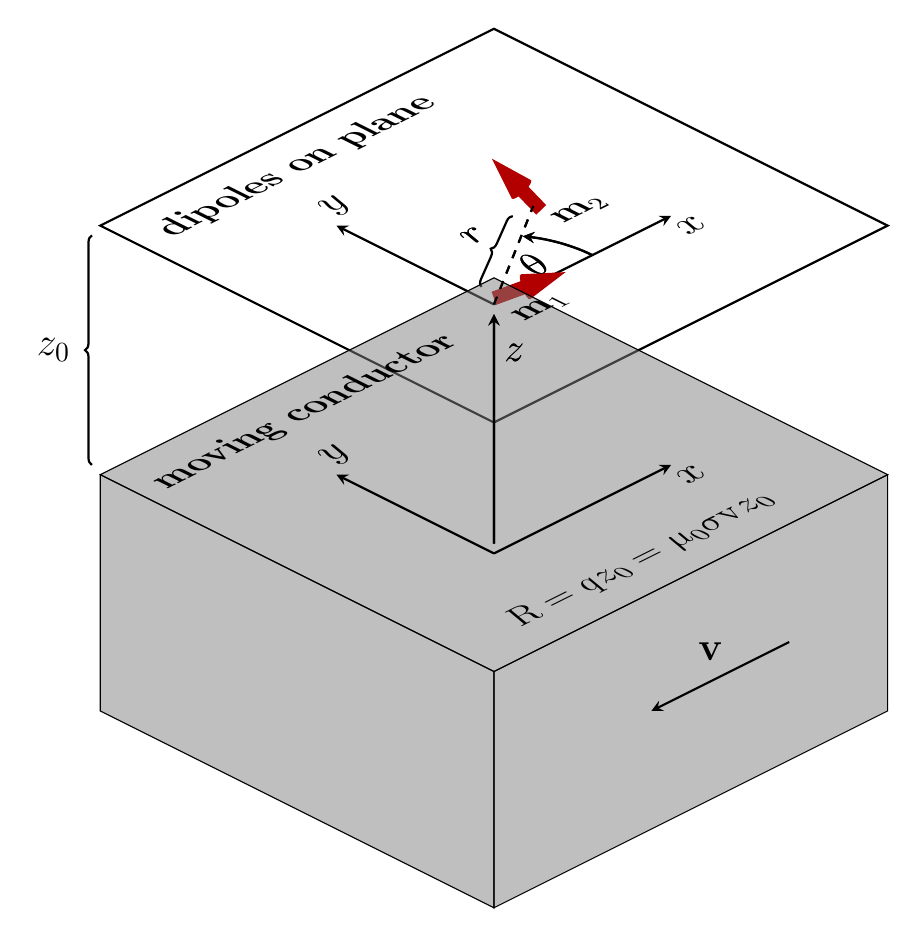
\begin{tikzpicture}

%%%%%%%%% FIRST LAYER - DIPOLES

 \begin{scope}
    [yshift=90,every node/.append style={
    	    yslant=0.5,xslant=-1},yslant=0.5,xslant=-1]
        \fill[white] (0,0) rectangle (5,5);
        \draw[black, thick] (0,0) rectangle (5,5);
      % \draw[step=5mm, black] (0,0) grid (5,5);
\draw[thick,decoration={brace,raise=5pt}, decorate] (1.65,1.65)--(2.75,2.35);
\draw[dashed, thick] (1.5,1.5)--(3,2.5);
\draw[thick, ->, >=stealth, ] (2.75, 1.5) arc [start angle=0,end angle=33,x radius=1.25,y radius=1.25];
  \draw[->, >=stealth, thick] (1.5,1.5)--(3.75,1.5);
\draw[->, >=stealth, thick] (1.5,1.5)--(1.5,3.5);

\node (Oz) at (1.5,1.5) {};
 \node (Cz) at (0,5) {};
 \node at (2.25,2.5) {\Large $r$};
 \node at (2.25,1.75) {\Large $\theta$};
 \node at (3.75,1.25) {\Large $x$};
 \node at (1.75,3.75) {\Large $y$};
% interacting dipoles
\draw[line width=5, color=darkred][-{Cone[pitch=15]}](1.,1., -1.5)--(1.5,1.1,-1.1);
\draw[line width=5, color=darkred][-{Cone[pitch=15]}](3,2.4, 0.)--(3.25,2.9,0.3);


%% other dipoles
%\draw[line width=5, color=darkgray][-{Cone[pitch=15]}](1.5,3.7, 0.)--(1.75,3.7,-0.5);
%\draw[line width=5, color=darkgray][-{Cone[pitch=15]}](1.5,2.45, 0.)--(1.5,2.45,-0.8);
%
%\draw[line width=5, color=darkgray][-{Cone[pitch=15]}](3,3.45, 0.)--(2.75,3.45,-0.8);
%\draw[line width=5, color=darkgray][-{Cone[pitch=15]}](3.05,1.65, 0.)--(2.85,1.15,-1);
%
%\draw[line width=5, color=darkgray][-{Cone[pitch=15]}](4.05,1.5, 0.)--(4.1,1.5,-0.8);
%\draw[line width=5, color=darkgray][-{Cone[pitch=15]}](4.15,2.45, 0.)--(4,2.45,-0.8);
%\draw[line width=5, color=darkgray][-{Cone[pitch=15]}](4,3.45, 0.)--(4.,3.45,-0.8);



\end{scope}
    	
 
 
%%%%%%%%% SECOND LAYER - CONDUCTOR

    \begin{scope}[
    	yshift=0,every node/.append style={
    	yslant=0.5,xslant=-1},yslant=0.5,xslant=-1]
    	\fill[gray,fill opacity=0.5] (0,0) rectangle (5,5);
    	\draw[black] (0,0) rectangle (5,5);
  % \draw[->, >=stealth, thick] (3.5,3) -- (2.,3);
  \draw[->, >=stealth, thick] (1.5,1.5)--(3.75,1.5);
\draw[->, >=stealth, thick] (1.5,1.5)--(1.5,3.5);
  \filldraw[fill=gray,fill opacity=0.5] (0.,5)--(-3,2)--(-3, -3)--(0, 0)--cycle;
    \filldraw[fill=gray, fill opacity=0.5] (0.,0)--(-3, -3)--(2, -3)--(5, 0)--cycle;

 
   \node (O) at (1.5,1.5) {};
  \node (C) at (0,5) {};

 \draw[->, >=stealth, thick] (2.25,-1.5) -- (0.5,-1.5);

 \node at (2.35,0.5) { \large $R=qz_{0}=\mu_{0}\sigma\mathrm{v}z_{0}$};


\end{scope}
 
\node at (2.75, 0.25) {\Large $\mathbf{v}$};

 \draw[thick, ->, >=stealth] (O) -- node[near end, above right] {\Large $z$}++(Oz);
 \draw[thick, decoration={brace,raise=3 pt}, decorate] (C) --node[left=0.25cm] { \Large  $z_{0}$} ++(Cz);


\begin{pgfonlayer}{foreground}
 \begin{scope}
    [yshift=90,every node/.append style={
    	    yslant=0.5,xslant=-1},yslant=0.5,xslant=-1]
 
 \draw[dashed, thick] (1.5,1.5)--(3,2.5);
\draw[thick, ->, >=stealth, ] (2.75, 1.5) arc [start angle=0,end angle=33,x radius=1.25,y radius=1.25];
 \node at (2.25,2.5) {\Large $r$};
 \node at (2.25,1.75) {\Large $\theta$};

 
\node at (1.75, 1.15)  {\large $\mathbf{m}_{1}$};  
\node at (3.25, 2.15)  { \large $\mathbf{m}_{2}$};  
 \node at (2,4.5) {\large \textbf{dipoles on plane }};

    \end{scope}
    
     \begin{scope}[
    	yshift=0,every node/.append style={
    	yslant=0.5,xslant=-1},yslant=0.5,xslant=-1]
      \node at (3.75,1.25) {\Large $x$};
      \node at (1.75,3.75) {\Large $y$};
 \node at  (2.1,4.5) {\large \textbf{moving conductor}};

    \end{scope}
     \draw[thick, ->, >=stealth] (O) -- node[near end, above right] {\Large $z$}++(Oz);
 \end{pgfonlayer}
  
\end{tikzpicture}
\end{document}